\chapter{First program}
\label{first-program}

Your first program to test your board should only flash an LED (the
hello world equivalent for embedded systems). The key to testing new
hardware is to have many programs that only do one simple task each.

Do not underestimate the effort required to flash your first LED. You
require:
%
\begin{itemize}
\item
  A computer with \program{git} installed and a useful shell program
  such as \program{bash}. UC has a
  \href{http://ucmirror.canterbury.ac.nz/}{mirror} for a variety of
  Linux distributions; we recommend Ubuntu or Mint.

\item A cloned copy of the Wacky Racers git repository, see
  \hyperref[project-cloning]{project cloning}.

\item
  A working ARM toolchain (arm-none-eabi-gcc/g++ version 4.9.3 or
  newer), see \hyperref[toolchain]{toolchain}.

\item
  An ST-link programmer and 10-wire ribbon cable for programming. You
  can get the adaptor from Scott Lloyd in the SMT lab. You will need
  to make your own cable (For a grey ribbon cable, align the red
  stripe with the small arrow denoting pin 1 on the connector. For a
  rainbow ribbon cable, connect the brown wire to pin 1.). There are
  two variants of the ST-link programmer with \textbf{different
  pinouts} so you may need to customise your programming cable.
\item
  Plenty of gumption.
\end{itemize}


Once you have a working toolchain and the source code installed:
%
\begin{enumerate}
\item Set up the PIO definitions for your board, see
  \hyperref[configuration]{configuration}.

\item Compile your program, see \hyperref[compilation]{compilation}.

\item See if your SAM4S is running, see \hyperref[openocd]{OpenOCD}.

\item Configure the SAM4s to boot from flash memory, see
  \hyperref[booting-from-flash-memory]{booting from flash memory}.

\item Program the SAM4s, see \hyperref[programming]{programming}.
\end{enumerate}


\begin{figure}
\chapter{OpenOCD}
\label{OpenOCD}

The Open On-Chip Debugger (OpenOCD) is an open-source on-chip
debugging, in-system programming, and boundary-scan testing tool. It
is able to communicate with various ARM and MIPS microprocessors via
\wikiref{JTAG}{JTAG} or \wikiref{SWD}{SWD}. It works with a number of
different \wikiref{JTAG}{JTAG} or \wikiref{SWD}{SWD}
interfaces/programmers. User interaction can be achieved via
\file{telnet/putty} or the GNU debugger (GDB).


\section{Configuration files}
\label{configuration-files}

OpenOCD needs a \wikiref{OpenOCD_configuration}{configuration file} to
specify the interface (USB or parallel port) and the target system.
Unfortunately, these change with every new release of OpenOCD.


\section{Running OpenOCD}
\label{running-openocd}

OpenOCD runs as a daemon program in the background and can be
controlled from other programs using TCP/IP sockets. This means that
you can remotely debug from another computer. The socket ports it uses
are specified in the \wikiref{OpenOCD_configuration}{OpenOCD
  configuration} file supplied when it starts. By default, OpenOCD
uses port 3333 for \wikiref{GDB}{GDB} and port 4444 for general
interaction using the \file{telnet} program.


\subsection{Communicating with OpenOCD using telnet}
\label{communicating-with-openocd-using-telnet}

If OpenOCD is running, commands can be sent to it using the telnet
program.  For example,
%
\begin{minted}{bash}
$ telnet localhost:4444
> halt
> at91sam4 info
\end{minted}
%
To exit use \code{ctrl-]} then \code{c}.  On Windows, you can use the
  \file{putty} program.


\subsection{Communicating with OpenOCD using GDB}
\label{communicating-with-openocd-using-gdb}

If OpenOCD is running, commands can be set to it with
\wikiref{GDB}{GDB}. There are two steps: connecting to OpenOCD with
the target remote command, and then sending a command with the GDB
monitor command. For example,

\begin{minted}{bash}
$ gdb
(gdb) target remote localhost:3333
(gdb) monitor flash info 0
\end{minted}

\section{OpenOCD commands}
\label{openocd-commands}

All the gory OpenOCD details can be found in the
\wikiref{Media:openocd.pdf}{OpenOCD manual}. If you are getting strange
errors see \wikiref{OpenOCD_errors}{OpenOCD errors}.

\section{Flash programming}
\label{flash-programming}

OpenOCD can program the flash program memory from a binary file.

%% \section{FTDI support}
%% \label{ftdi-support}

%% Many \wikiref{JTAG_interface}{JTAG interfaces} use chips made by Future
%% Technology Devices International (FTDI) to translate between the USB and
%% JTAG protocols. FTDI provide a library to communicate with these
%% devices; however, this is not open-source and hence cannot be
%% distributed. There is an open-source equivalent,
%% \href{http://freshmeat.net/projects/libftdi/}{libftdi}, which in turn
%% uses the open-source libusb. This can be temperamental to get working on
%% a Windows system.

%% \section{Getting OpenOCD}
%% \label{getting-openocd}

%% The developers of OpenOCD release source packages (and provide
%% subversion access) but do not provide official builds for any
%% operating system. However, there are various sites which provide
%% pre-built versions of OpenOCD.

%% \subsection{Windows}
%% \label{windows}

%% Windows installers for release versions of OpenOCD can be found
%% \href{http://www.freddiechopin.info/index.php/en/download/category/4-openocd}{here}.
%% Some development versions can be found
%% \href{http://www.freddiechopin.info/index.php/en/download/category/10-openocd-dev}{here}.
%% Unless you need a feature not present in the release version, avoid
%% getting the development versions as they can be less stable.

%% Alternatively, the
%% \href{http://www.siwawi.arubi.uni-kl.de/avr_projects/arm_projects/}{WinARM}
%% toolchain contains a version of OpenOCD, albeit one that appears (from
%% the description on the project page) to be out of date. It is also
%% possible to build your own copy of OpenOCD using either
%% \href{http://www.mingw.org/}{MinGW} or
%% \href{http://www.cygwin.com/}{Cygwin}; instructions for this are posted
%% in various places online.

%% Realistically, it's probably easier to set up a virtual machine with
%% Linux and use that instead.

%% \subsection{Linux}
%% \label{linux}

%% Many recent distributions of Linux have OpenOCD in their software
%% repositories. However, this is often out of date and (in some cases)
%% buggy. In this case it is straightforward to
%% \wikiref{Building_OpenOCD_under_Linux}{build the latest version}.

%% \subsection{Mac OSX}
%% \label{mac-osx}

%% The easiest way to install OpenOCD on Mac OSX is to use
%% \href{http://brew.sh/}{Homebrew}. If you wish to use JTAG with an
%% adaptor based on a FTDI chip (for example, the UCECE USB to JTAG
%% adaptor or a Bus Blaster), make sure you include libftdi support by
%% installing with the command:
%% %
%% \begin{minted}{bash}
%% $ brew install openocd --enable-ft2232_libftdi
%% \end{minted}

\section{System information}
\label{system-information}


The openocd command \code{at91sam4 info}, see
\hyperref[communicating-with-openocd-using-telnet]{communicating with
  OpenOCD using telnet}, outputs useful information about the state of
the SAM4S.  For example:
%
\begin{verbatim}
    CKGR_MOR: [0x400e0420] -> 0x01006409
	    MOSCXTEN:     1 [0x0001] (main xtal enabled: YES)
	    MOSCXTBY:     0 [0x0000] (main osc bypass: NO)
	    MOSCRCEN:     1 [0x0001] (onchip RC-OSC enabled: YES)
	     MOSCRCF:     0 [0x0000] (onchip RC-OSC freq: 4 MHz)
	    MOSCXTST:   100 [0x0064] (startup clks, time= 3051.757812 uSecs)
	     MOSCSEL:     1 [0x0001] (mainosc source: external xtal)
	       CFDEN:     0 [0x0000] (clock failure enabled: NO)
   CKGR_MCFR: [0x400e0424] -> 0x000117ac
	    MAINFRDY:     1 [0x0001] (main ready: YES)
	       MAINF:  6060 [0x17ac] (12.411 Mhz (32.768khz slowclk)
  CKGR_PLLAR: [0x400e0428] -> 0x08133f01
	        DIVA:     1 [0x0001]
	        MULA:    19 [0x0013]
	PLLA Freq: 248.218 MHz
   CKGR_UCKR: [0x400e041c] -> 0x00000000
    PMC_FSMR: [0x400e0470] -> 0x00000000
    PMC_FSPR: [0x400e0474] -> 0x00000000
     PMC_IMR: [0x400e046c] -> 0x00000000
    PMC_MCKR: [0x400e0430] -> 0x00000012
	         CSS:     2 [0x0002] plla (248.218 Mhz)
	        PRES:     1 [0x0001] (clock/2)
		Result CPU Freq: 124.109
    PMC_PCK0: [0x400e0440] -> 0x00000000
    PMC_PCK1: [0x400e0444] -> 0x00000000
    PMC_PCK2: [0x400e0448] -> 0x00000000
    PMC_PCSR: [0x400e0418] -> 0x41004000
    PMC_SCSR: [0x400e0408] -> 0x00000001
      PMC_SR: [0x400e0468] -> 0x0003000f
 CHIPID_CIDR: [0x400e0740] -> 0x289c0ae0
	     Version:     0 [0x0000]
	       EPROC:     7 [0x0007] Cortex-M4
	     NVPSIZE:    10 [0x000a] 512K bytes
	    NVPSIZE2:     0 [0x0000] none
	    SRAMSIZE:    12 [0x000c] 128K Bytes
	        ARCH:   137 [0x0089] ATSAM3S/SAM4S xB Series (64-pin version)
	      NVPTYP:     2 [0x0002] embedded flash memory
	       EXTID:     0 [0x0000] (exists: NO)
 CHIPID_EXID: [0x400e0744] -> 0x00000000
   rc-osc: 4.000 MHz
  mainosc: 12.411 MHz
     plla: 248.218 MHz
 cpu-freq: 124.109 MHz
mclk-freq: 124.109 MHz
 UniqueId: 0x53343100 0x50524a46 0x36303430 0x30363030
\end{verbatim}
%
Note, the reported clock frequencies are not accurate.


\section{Errors}
\label{openocd_errors}

\verb+Error: libusb_open() failed with LIBUSB_ERROR_ACCESS+ On Linux
you need to give permissions to access the USB.  You can do this by
finding the file \file{99-openocd.rules} that comes with the OpenOCD
distribution and then:
%
\begin{minted}{bash}
  $ sudo cp 99-openocd.rules /etc/udev/udev.rules
  $ sudo udevadm control --reload
\end{minted}
%
Finally, you need to reconnect the ST-link device.


See also \wikiref{OpenOCD_errors}{OpenOCD errors}.


\section{Programming without GDB}

OpenOCD can program the SAM4S without using GDB.  You will need to
kill any currently running instance of OpenOCD and then use:
%
\begin{minted}{bash}
  $ openocd -f path-to-sam4s-stlink.cfg -c "program program.bin verify reset exit"
\end{minted}
%
Here \file{program.bin} is the name of the program to load.

\caption{How OpenOCD interacts with the debugger and the SAM4S.}
\label{fig:openocd diagram}
\end{figure}


\section{Connecting with OpenOCD}
\label{openocd}

\begin{figure}[!h]
  \centering 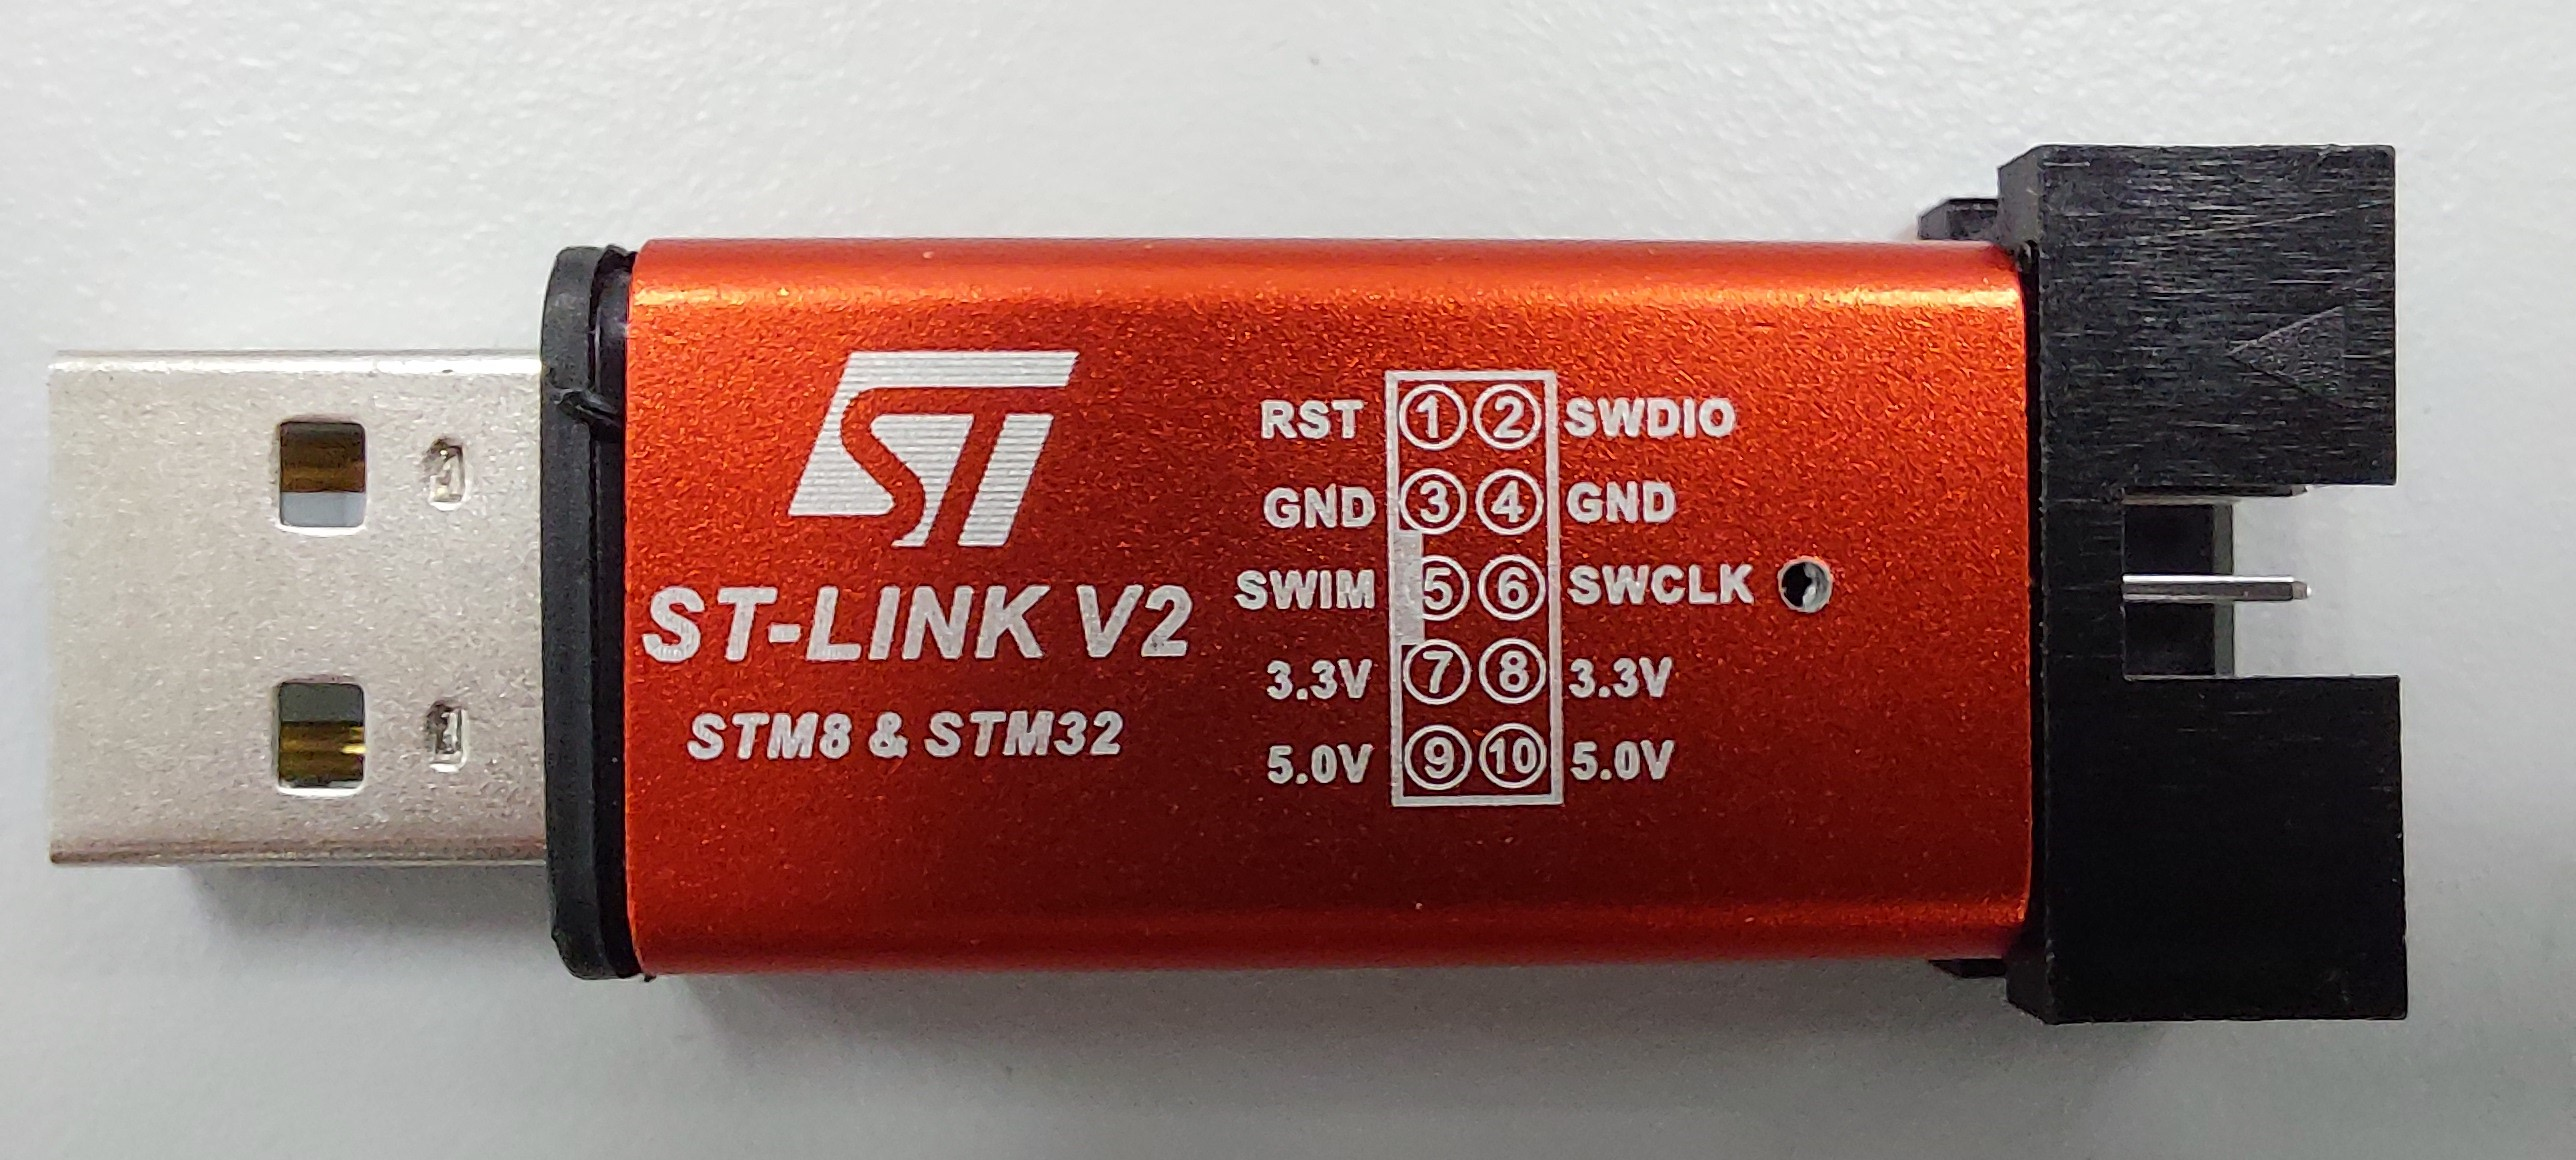
\includegraphics[width=4in]{figs/stlink.jpg}
  \caption{A Chinese copy of a ST-link programmer.  Unfortunately, the
    manufacturer is not consistent with the pinout!}
  \label{fig:stlink}
\end{figure}


\program{OpenOCD} is used to program the SAM4S, see \reffig{openocd diagram}.

For this assignment, we use a ST-link programmer to connect to the
SAM4S using serial wire debug (SWD). This connects to your board with
a 10-wire ribbon cable and an IDC connector.

\begin{enumerate}
\item
  Before you start, disconnect the battery and other cables from your
  PCB.
\item
  Connect a 10-wire ribbon cable from the ST-link programmer to the
  programming header on your PCB. This will provide 3.3\,V to your
  board so your green power LED should light.
\item
  Open a \textbf{new terminal window, e.g., bash} and
  start \program{OpenOCD}.
\end{enumerate}

\begin{minted}{bash}
$ cd wacky-racers
$ openocd -f src/mat91lib/sam4s/scripts/sam4s_stlink.cfg
\end{minted}

All going well, the last line output from \program{OpenOCD} should be:

\begin{verbatim}
Info : sam4.cpu: hardware has 6 breakpoints, 4 watchpoints
\end{verbatim}

Congrats if you get this! It means you have correctly soldered your
SAM4S. If not, do not despair and do not remove your SAM4S. Instead,
see \protect\hyperref[troubleshooting]{troubleshooting}.


\section{LED flash program}
\label{led-flash-program}

For your first program, use
\wfile{test-apps/ledflash1/ledflash1.c}. The macros \code{LED1_PIO}
and \code{LED2_PIO} need to be defined in \file{target.h} (see
\protect\hyperref[configuration]{configuration}).

\inputminted{C}{../../src/test-apps/ledflash1/ledflash1.c}

If the LED does not flash see \hyperref[debugging-LED]{debugging LED}.
If the LED does not flash at 2\,Hz, try the \hyperref[pwm-test]{PWM
  test} program and check the frequency with an oscilloscope.  If the
frequency is not 100\,kHz, the chief culprit is the PLL in the SAM4S.


\section{Configuration}
\label{configuration}

Each board has different PIO definitions and requires its own
configuration information. The \wfile{boards} directory contains a
configuration for the hat and one for the racer board.  \textbf{You
must edit these to customise your board.}  Each configuration
directory contains three files:

\begin{itemize}
\item
  \file{board.mk} is a makefile fragment that specifies the MCU model,
  optimisation level, etc.
\item
  \file{target.h} is a C header file that defines the PIO pins and
  clock speeds.
\item
  \file{config.h} is a C header file that wraps target.h. Its purpose
  is for porting to different compilers.
\end{itemize}

\textbf{You will need to edit the target.h file for your board} and set
the definitions appropriate for your hardware. Here's an excerpt from
\file{target.h} for a hat board:

\begin{minted}{C}
/* USB  */
#define USB_VBUS_PIO PA5_PIO

/* ADC  */
#define ADC_BATTERY PB3_PIO
#define ADC_JOYSTICK_X PB2_PIO
#define ADC_JOYSTICK_Y PB1_PIO

/* IMU  */
#define IMU_INT_PIO PA0_PIO

/* LEDs  */
#define LED1_PIO PA20_PIO
#define LED2_PIO PA23_PIO
\end{minted}


\section{Compilation}
\label{compilation}

Due to the many files required, compilation is performed using
makefiles.

The demo test programs are generic and you need to specify which board
you are compiling them for. The board configuration file can be chosen
dynamically by defining the environment variable \code{BOARD}. For
example:
%
\begin{minted}{bash}
$ cd src/test-apps/ledflash1
$ BOARD=racer make
\end{minted}

If all goes well, you should see at the end:
%
\begin{verbatim}
   text    data     bss     dec     hex filename
  11348	   2416	    176	  13940	   3674	ledflash1.bin
\end{verbatim}

To avoid having to specify the environment variable \code{BOARD}, you
can define it for the rest of your session using:
%
\begin{minted}{bash}
$ export BOARD=racer
\end{minted}
%
and then just use:
%
\begin{minted}{bash}
$ make
\end{minted}

\section{Booting from flash memory}
\label{booting-from-flash-memory}

By default the SAM4S runs a bootloader program stored in ROM. The SAM4S
needs to be configured to run your application from flash memory.

If \program{OpenOCD} is running you can do this with:

\begin{minted}{bash}
$ make bootflash
\end{minted}

Unless you force a complete erasure of the SAM4S flash memory by
connecting the \pin{ERASE} pin to 3.3\,V, you will not need to repeat
this command.

\section{Programming}
\label{programming}

If \program{OpenOCD} is running you can store your program in the flash
memory of the SAM4S using:

\begin{minted}{bash}
$ make program
\end{minted}

When this finishes, one of your LEDs should flash. If so, congrats! If
not, see \protect\hyperref[troubleshooting]{troubleshooting}.

To reset your SAM4S, you can use:
%
\begin{minted}{bash}
$ make reset
\end{minted}


\section{Makefiles}

Compilation is performed using makefiles, since each application
requires many files.  Rather than having large makefiles, a heirarchy
of makefile fragments is employed.  Dependencies are automatically
generated (so not all the files have to be recompiled each time).

A board description can be selected with the \code{BOARD} environment
variable.  This can be defined for each command, for example,
%
\begin{minted}{bash}
$ BOARD=racer make program
\end{minted}


Alternatively, this can be defined for a session:
%
\begin{minted}{bash}
$ export BOARD=racer
$ make program
\end{minted}


Each of the makefiles has the following phony targets:
%
\begin{description}
\item[all]  --- compile the application
\item[program] --- compile the application and download to the MCU (you need Openocd running)
\item[debug] --- start the debugger GDB (you need Openocd running)
\item[reset] --- reset the MCU (you need Openocd running)
\item[clean] --- delete the executable, object files, and dependency files.
\end{description}
